\documentclass{article}
\usepackage[margin=0.5in]{geometry}
\usepackage[utf8]{inputenc}
\usepackage{listings}
\usepackage{amsmath}
\usepackage{graphicx}
\usepackage{setspace}
\title{CS-520 Assignment 1}
\author{Sri Vamsi Kalyan Peta(SP2267), Nitish Kumar Thottempudi(NT451),\\Sai Govardhan Reddy Kanjula(SK2674)}
\date{October 2022}

\newcommand\tab[1][1cm]{\hspace*{#1}}
\begin{document}

\maketitle
\setlength{\parindent}{20pt}
\section*{Part 0}
Steps Implemented in Maze generation using the DFS approach with random tie-breaking
\begin{enumerate}
    \item Generated maze using DFS by using random tie-breaking as required
    \item Maze is created using a 2-dimensional array with block and unblocked status stored using a boolean value
    \item The maze is initialized as unblocked for all the cells and a similar size of the 2-dimensional matrix is created for keeping track of the visited cells in 1st matrix
    \item A vector stack same as the size of the maze is also created to record the visited cells of the maze and resized to double when its full
    \item Firstly, we select a random cell and randomly select on of its unvisited neighbors as either blocked/unblocked with a probability of 0.3 for blocked and 0.7 for unblocked. We then push the cell to stack and mark it as visited, we repeat this until we discover a dead end. Once, we reach the dead end, we keep popping the cells until we find a cell, which has unvisited neighbors. All the cells are considered visited if the stack is empty
\end{enumerate}
\begin{lstlisting}[title=Maze generation using DFS approach with random tie-breaking]
Initializing maze M = {False} -> all cells unvisited
            MarkupMaze N = {False} -> all cells unvisited
            Stack = Empty stack to push and pop visited cells
            StartPoint = A0
            Probability of Block Generation = pb

stack.push(A0)
N(A0) = True
While !stack.empty() 
    A_current = stack.top() 
    #Randomly select a neighbor of A_current
    if neighbour exists -> A_next
        set M(A_next) = True #(with pb)
        N(A_next) = True
        if stack is full:
            #increase the capacity of stack by double
        end if
    stack.push($A_next$)
    else
        stack.pop()
    end if
end while
return Maze M
\end{lstlisting}

\section*{Part 1}
\renewcommand{\labelenumi}{\alph{enumi})}
\begin{enumerate}
    \item In repeated $A^*$\ search, the agent initially knows that its neighbor cells $E_1$, $D_2$, and $E_3$ are unblocked.\\
    Now the agent calculates the F(n) for all its neighbor cells to identify the cell that has the least F(n) to make its next move\\
    By calculating F(n) for $E_1$, $D_2$, $E_3$\\
    F($E_1$) = 5\\
    F($D_2$) = 5\\
    F($E_3$) = 3\\
    Since the F Value of $E_3$ is smaller compared to all the neighbors, the agent first moves to the east rather than the north
    \item To Prove that the agent in a finite grid world either reaches the target or discovers that this is impossible in finite time, let's consider 2 cases
    \begin{description}
    \item[case 1:]Let's consider that the target is not separated by blocked cells. In this case, at every instance, when the blocked cell is discovered, the $A^*$ algorithm can always find a path from the cell that the agent is currently in to the target cell. The agent is guaranteed to reach the target in the given finite grid world.
    \item[case 2:] Now, let's consider that the target is separated by blocked cells. The agent makes at least one movement every time the $A^*$ algorithm finds the path and ends up knowing more about the grid world. In the worst case, the agent knows the entire grid world in finite time, while the $A^*$ algorithm cannot find the path to the target, the agent is very well known that it is impossible to reach the target.
    \end{description}
    To prove the number of moves of the agent until it reaches the target or discovers that it is impossible is bounded from above by the number of unblocked cells squared. Let's consider 2 cases.
    \begin{description}
    \item[case 1:] The target is not separated by blocked cells. Given n blocked cells in the path from the agent to the target, the path contains almost n-1 states. In the worst-case scenario let's assume that the agent encounters a blocked cell every time. Due to the optimality of $A^*$ search, the same cell is not present in every search. $A^*$ search is bounded by $(n-1)$ moving states and the total moves, therefore, is almost $(n-1)^2$, which is less than $n^2$
    \item[case 2:] The target is separated by blocked cells. In this case, the path doesn't exist from agent to target. Here the agent should explore all the unblocked states that can be reached from the start state. before determining that the path doesn't exist. The number of such unblocked states is bounded by $(n-1)$ and the agent can make at most $(n-2)$ moves to find an unblocked state. clearly, $(n-1)(n-2)$ $<$ $n^2$.
    \end{description}
    Therefore number of moves is bounded by the square of no of blocked states.
\end{enumerate}

\section*{Part 2}
\begin{figure}[h!]
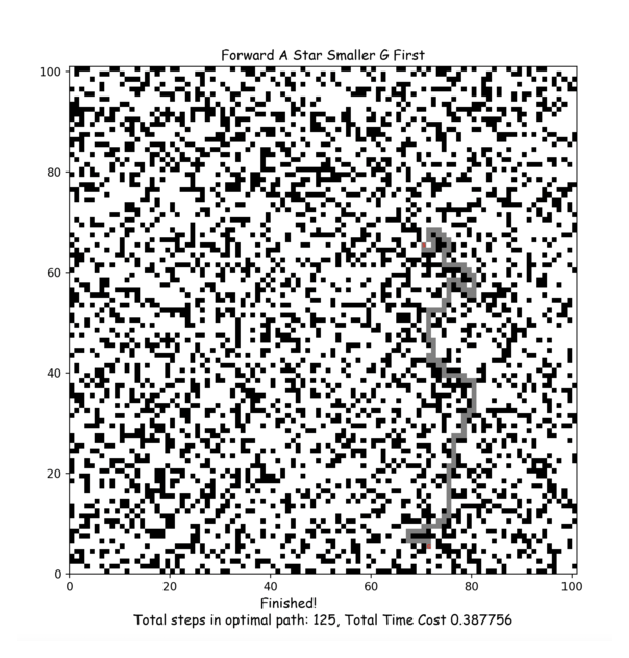
\includegraphics[width=0.5\textwidth, inner]{fsmg1}
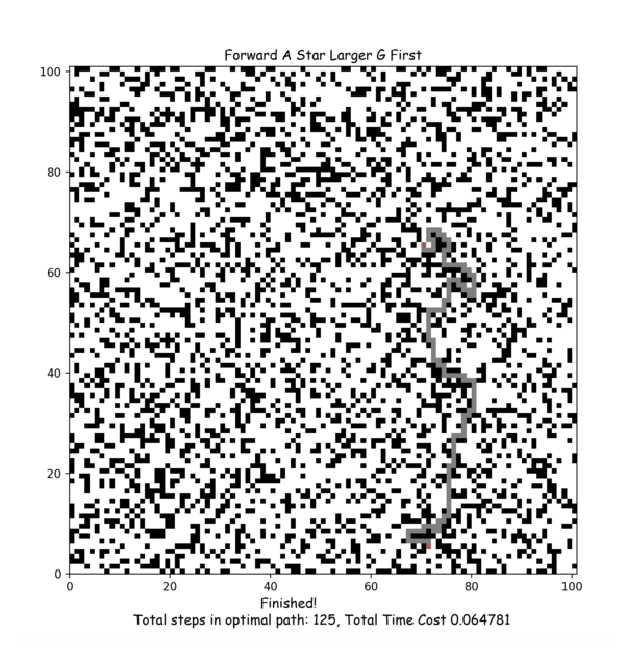
\includegraphics[width=0.5\textwidth, right]{flg1}
\caption{Smaller G First Vs Larger G First}
\label{fig:figure2}
\end{figure}
\noindent Theoretically speaking, although there is a probability for all possible sort of outcomes. As per the observations, we've made with statistical significance on an average over the multiple generated mazes. We have 
identified with the highest probability that breaking ties by selecting the agent with larger g value expands fewer cells than the agent with 
small g value.\\
\\
As per our analysis, the main reason for the lesser cell expansion with a larger g value is that the larger g value prompts the $A^*$  to follow a 
single path, whereas, in the case of smaller g values, $A^*$ is prompted to take a way back to expand the cells in proximity to start cell. This makes up for costing many unnecessary expansions in the case of smaller g values.\\
\\
Therefore, $A^*$ in favor of larger g values is the best for breaking ties.\\
\section*{Part 3}
As per observations and outcomes of our implementation on an average over multiple samplings with statistical significance, we identified that forward $A^*$ most probably has fewer cell expansions compared to the backward $A^*$ algorithms. The result of fewer cell expansions, forward $A^*$ takes less execution time compared to backward $A^*$.\\
\\
In the case of forwarding $A^*$, the agent only knows about the cells near the start cell, whereas in backward $A^*$, before reaching the block near the start cell, the f values of the cells in the open list are the same as the Manhattan distance from start cell to the target. This is also equal to the smallest f value in the search. It is highly possible that the distance of the path from start to target is greater than their Manhattan distance. With the increase in f value, it expands cells within smaller f values in the open list by going back, resulting in the cell expanding many more cells with smaller f values.
\\
Backward $A^*$ expands cells with smaller f-values and later expands the larger f-value cells.\\
\\
In contrast the forward $A^*$ increases its f value in the initial steps to maintain the same f value till the goal state is reached. with an increase in the f value of a current cell, very few states are left with smaller f value in the open list because of the reason that very few states are searched and blocked cells in the proximity excludes many to be searched.\\
Therefore forward $A^*$ makes substantially fewer expansions compared to the backward $A^*$ and thereby resulting in less execution time in forward $A^*$\\
\begin{figure}[h!]
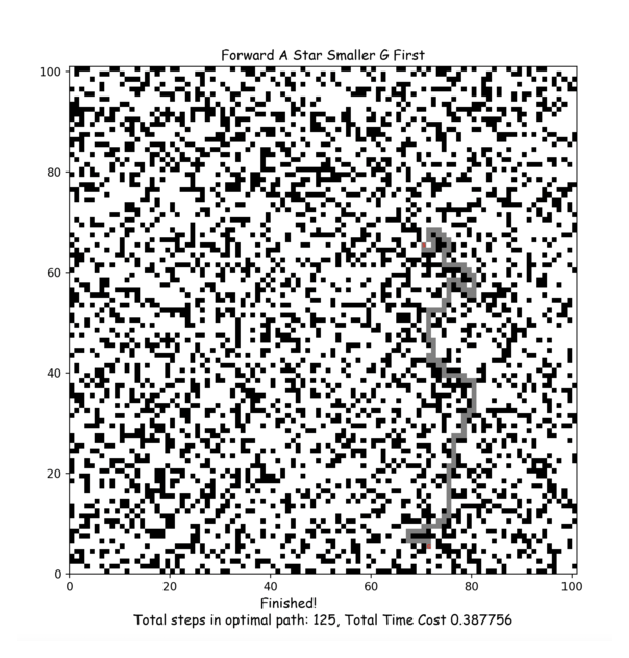
\includegraphics[width=0.5\textwidth, inner]{fsmg1}
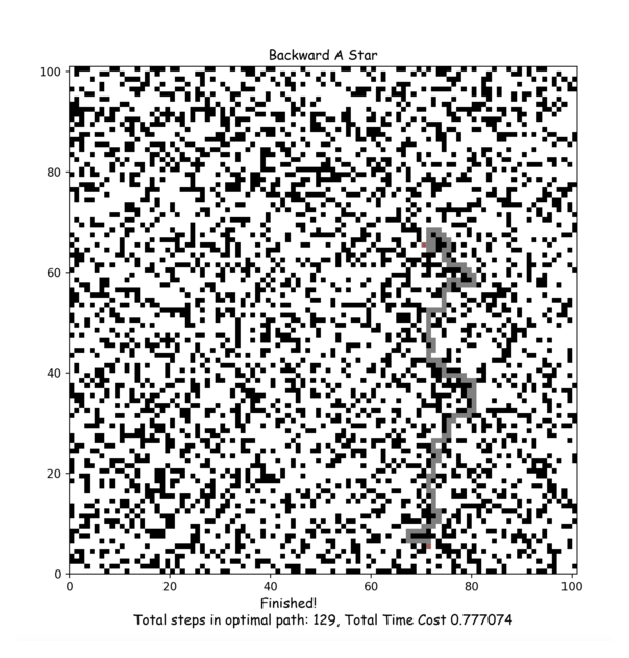
\includegraphics[width=0.5\textwidth, right]{fg1}
\caption{Forward $A^*$ Vs Backward $A^*$}
\label{fig:figure2}
\end{figure}

\section*{Part 4}
$h(s)$ = Manhattan distance between states and $s_{goal}$\\
if s = $s_{goal}$,\\
\tab $h(s_{goal}) = |x_{Sgoal} - x_{Sgoal}| + |y_{Sgoal} - y_{Sgoal}| = 0$\\
\tab where $x_s$ and $y_s$ are indexes of rows and columns for states\\
if s != $s_{goal}$\\
\tab let n = succ(s,a)\\
\tab then, $h(s)-h(n) = |x_s - x_{Sgoal}| + |y_s - y_{Sgoal}| - |x_n - x_{Sgoal}| + |y_n - y_{Sgoal}|$\\
since s and n are neighbors in grids and the agent can only move in 4 main compass directions,\\
we have $x_s=x_n or y_s=y_n$\\
if $x_s=x_n$ then\\
\tab $|y_s-y_n| = 1$\\
In the above case $h(s)-h(n) = |y_s - y_sgoal| - |y_n - y_sgoal| \leq |y_s - y_n| = 1$\\
\\
if $y_s=y_n$ then\\
\tab $h(s) - h(n) \leq |x_s-x_n| = 1$\\
In both cases, $h(s) - h(n) \leq 1 = c(s,a)$\\
$=>$ h(s) \leq h(succ(s,a)) + c(s,a)$\\
Therefore the Manhattan distances are consistent in grid worlds where agent can move only in 4 main compass directions.\\

\noindent b) Prove that Adaptive $A^*$ leaves initially consistent h-values consistent even if action cost can increase.

\noindent In adaptive $A^*$, there are 3 cases for h-value of states and its successive state $succ(s,a)- >n$\\
\begin{description}
\item[case 1:] s and n were expanded in last search. Here, heuristics of both state s and n are defined new.\\
\begin{spacing} {0.7}
$h_{new}(s) = g(s_{goal})-g(s)$\\
\end{spacing}
$h_{new}(n) = g(s_{goal}) - g(n)$\\
\\
$A^*$ search find a trajectory from current state through state s to state n of cost $g(s) + c(s,a)$\\
This cost may not be the final g value of state n due to the possibility of a shorter path\\
Therefore $g(n) \leq g(s) + c(s,a)$
\\
$h_{new}(s) = g(s_{goal}) - g(s) \leq g(s_{goal}) - g(n) + c(s,a) = h_{new}((n) + c(s,a)$
\item[case 2:] State s was expanded but state n was not in last search.\\
Here, the h-value of s is defined new.\\
\tab $h_{new}(s) = g(s_{goal}) - g(n)$\\
But state n is still Manhattan distance to target\\
$h_{new}(n) = h(n)$\\
we know that $g(n) \leq g(s) + c(s,a)$ - from case 1\\
state n is generated but not expanded\\
f-value of n is not smaller than s\\
\begin{math}
F(s) \leq F(n)\notag\\
Therefore, h_{new}(s) = g(s_{goal}) - g(s)\notag\\
\tab \tab \tab =F(s_{goal}) - g(s) \leq F(s) - g(s)\notag\\
\tab \tab \tab F(n) - g(s) = g(n) + h(n) -g(s)\notag\\
\tab \tab \tab =g(n) + h_{new}(n) - g(s) \leq g(n) + h_{new}(n) - g(n) + c(s,a)\notag\\
\tab \tab \tab =h_{new}(n) + c(s,a)
\end{math}

\item[case 3:] State s - not expanded in last search,\\
Here, $h_new(s) = h(s)$\\
Heuristics of same state are monotonically increasing over time,\\
Therefore, $h(n) \leq h_new(n)$\\
$=> h_{new}(s) = h(s) \leq h(n)+c(s,a)<=h_new(n)+c(s,a)$\\
New h-values are consistent even if the action costs can increase\\
\end{description}

\section*{Part 5}
As per our observations, Adaptive A* outperforms repeated forward $A^*$ with the highest probability in terms of the number of cells expanded during the search\\

\noindent The main reason, we have identified for the lesser expansions in adaptive $A^*$ compared forward $A^*$ is that in adaptive A*, the h-values of states in (n-1)th  adaptive $A^*$ are updated with the real paths from those states to the target while moving from path obtained from (n-1)th adaptive A*. Utilization of updated h-values which reflects their accurate distances results in fewer expansions than the Manhattan distances. A state that has the smallest Manhattan distance to the target can possibly have greater h-values, given that all paths having a length of manhattan lengths are blocked. Leveraging on these updated h-values can result in avoiding the expansion of states with higher h-values but small Manhattan distances whereas repeated forward $A^*$ will probably expand those states. Therefore adaptive $A^*$ will expand no more excess states compared to repeated forward $A^*$.\\

\noindent Although Theoretically adaptive $A^*$ is meant to have fewer expansions in comparison to repeated forward A*, there are few cases where adaptive A* expands more states. This situation arises due to the priority queue, which is implemented using a binary heap. The FIFO role doesn’t always hold place when states with the same f and g values are put into the queue. In such cases, adaptive a* may expand upon another path that has the same cost as forward A*. The placement of blocks along the path makes adaptive A* do more repetitions going forward than forward $A^*$, resulting in more expanded states and execution time compared to forward $A^*$.\\ 

%...
\begin{figure}[h]
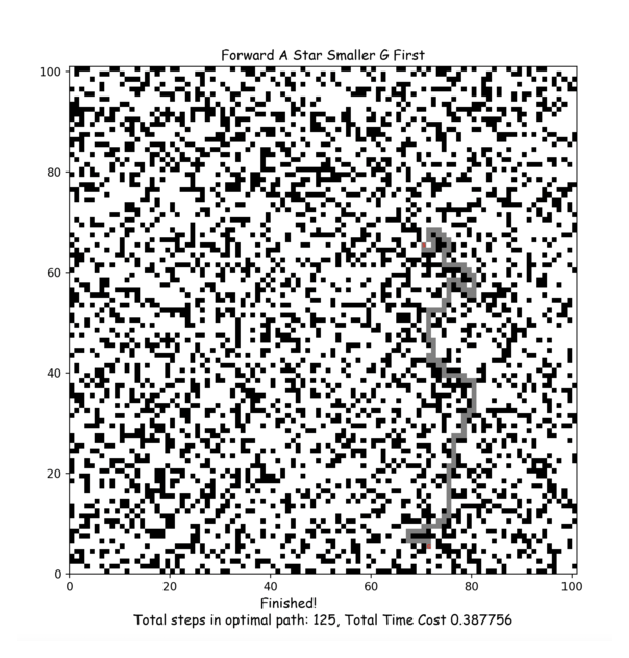
\includegraphics[width=0.5\textwidth, inner]{fsmg1}
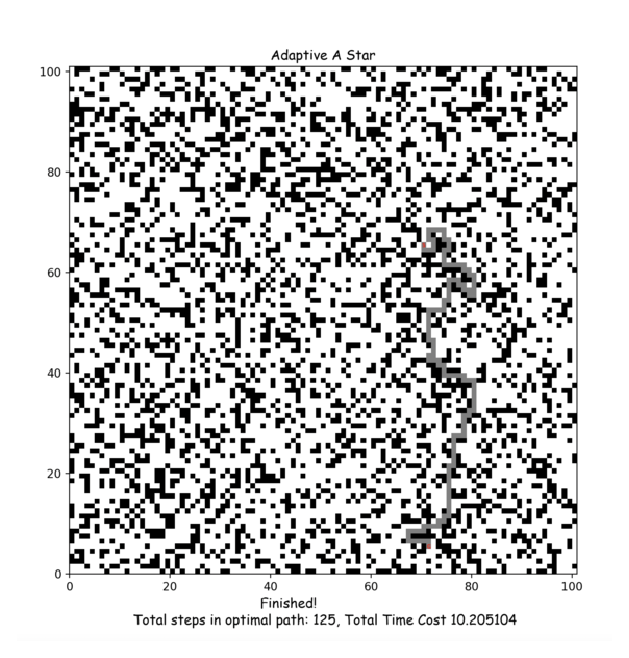
\includegraphics[width=0.5\textwidth, right]{b}
\caption{Forward $A^*$ Vs Adaptive $A^*$}
\label{fig:figure2}
\end{figure}


\section*{Part 6}

Using just execution time to compare the algorithms is a biased measure of performance. Let’s take Part 3 for reference where we compare the Repeated Forward A* algorithm and the Repeated backward A* algorithm. Let’s obtain the data for statistics from running a few test cases. Now we calculate the median for the run data obtained through multiple tests (we can’t use mean as it can get affected by the extreme data points). We can find which algorithm is better if there is a notable difference in run time. Else we can use some other parameter like the number of tasks in an algorithm or the number of processors. We know run time is a dependent variable whereas the number of jobs and number of processors is independent.\\

\noindent So, let's assume
Null Hypothesis$(H_0)$:  Repeated backward A* algorithm and Repeated Forward A* algorithm have a systematic performance difference.\\
Alternate Hypothesis$(H_1)$: We can’t express the performance difference in a systematic nature for the above algorithms.\\

\noindent 1) Get the data from multiple test cases\\
2) Find the distribution of standard differences under the assumption that they can be expressed as a linear function\\
3) Using this premise calculate the probability of deviation\\
4) If the probability is very low then our alternate hypothesis is false\\

\noindent We are using Statistical Hypothesis testing for the above case.


\end{document}


